%\documentclass{beamer}            %% interactive
\documentclass[handout]{beamer}   %% handouts
\usepackage{graphicx}
\usepackage{bbm}
\usepackage{amsmath}
\usepackage{amssymb}
\usepackage[utf8]{inputenc}
\usepackage{tikzsymbols}
\usepackage{hyperref}
%\usepackage{listings}
\usepackage[polish]{babel}
\usepackage[plmath,T1]{polski}

\def\cp#1{\textbf{\color{purple}{#1}}}
\def\R{\mathbb{R}}
\def\N{\mathbb{N}}
\def\C{\mathbb{C}}
\def\K{\mathbb{K}}
\def\S{S}
\def\M{\mathcal{M}}
\def\1{\mathbbm{1}}
\def\L{\mathcal{L}}
\def\X{\mathcal{X}}
\def\argmin{\mathop{\rm arg\,min}\limits}
\def\argmax{\mathop{\rm arg\,max}\limits}
\def\b#1{{\bf #1}}

\newcommand\blfootnote[1]{%
  \begingroup
  \renewcommand\thefootnote{}\footnote{#1}%
  \addtocounter{footnote}{-1}%
  \endgroup
}
\newcommand\graphics[1]{%
  \blfootnote{\hbox{}\hskip-0.6cm Graphics: \url{#1}}%
}


\usetheme{Warsaw}
\title[SVM]{Support Vector Machines\\
  and Kernels}
\author{Krzysztof Czarnowski}
\date{v2, May 22, 2017}

\begin{document}


%%%%%%
\begin{frame}
  \titlepage
\end{frame}


%%%%%%
\begin{frame}{Plan for today}
  \begin{itemize}
  \item Linear classification and linear SVM.
  \item Convex optimization and duality.
  \item Features, kernels and kernel trick.
  \item Nonlinear (kernel) SVM.
  \item Other kernel methods
  \item Examples
  \item Some diversions\/\dots (?)
  \item Not today:
    \begin{itemize}
    \item In depth theory of kernels and RKHS.
    \item VC-dimension and statistical theory of learning
      \item More omitions\/\dots
    \end{itemize}
  \end{itemize}
\end{frame}


%%%%%%
\begin{frame}{Linear classifiers}
  \begin{itemize}
  \item Naive, based on class means \\
    --- why it's not the best possible one.
  \item Fisher classifier --- the celebrated classics! LDA.
  \item Linear SVM.
  \item Underlying optimization scheme.
  \end{itemize}
\end{frame}




%%%%%%
%%\begin{frame}[fragile]\frametitle{Linear classifiers, toy datasets}
%%  We generate some samples from gaussian distributions:
%%  \begin{itemize}
%%  \item the ``blue's''\dots
%%\begin{verbatim}
%%mean1 = [1.0, 1.0]; cov1 = [[1.0, 0.0], [0.0, 1.0]]
%%NV1 = stats.multivariate_normal(mean1, cov1)
%%\end{verbatim}
%%  \item the ``green's''\dots
%%\begin{verbatim}
%%mean2 = [-1.0, 1.0]; cov2 = [[0.3, 0.0], [0.0, 2.0]]
%%NV2 = stats.multivariate_normal(mean2, cov2)
%%\end{verbatim}
%%  \item the ``yellow's''\dots
%%\begin{verbatim}
%%mean3 = [-1.0, -1.0]; cov3 = [[2.0, 0.0], [0.0, 2.0]]
%%NV3 = stats.multivariate_normal(mean3, cov3)
%%\end{verbatim}
%%  \item and the ``red's''
%%\begin{verbatim}
%%mean4 = [1.0, -1.0]; cov4 = [[0.6, 0.0], [0.0, 4.0]]
%%NV4 = stats.multivariate_normal(mean4, cov4)
%%\end{verbatim}
%%  \end{itemize}
%%\end{frame}


%%%%%%
\begin{frame}{Example 1: symmetric gaussian distributions}
  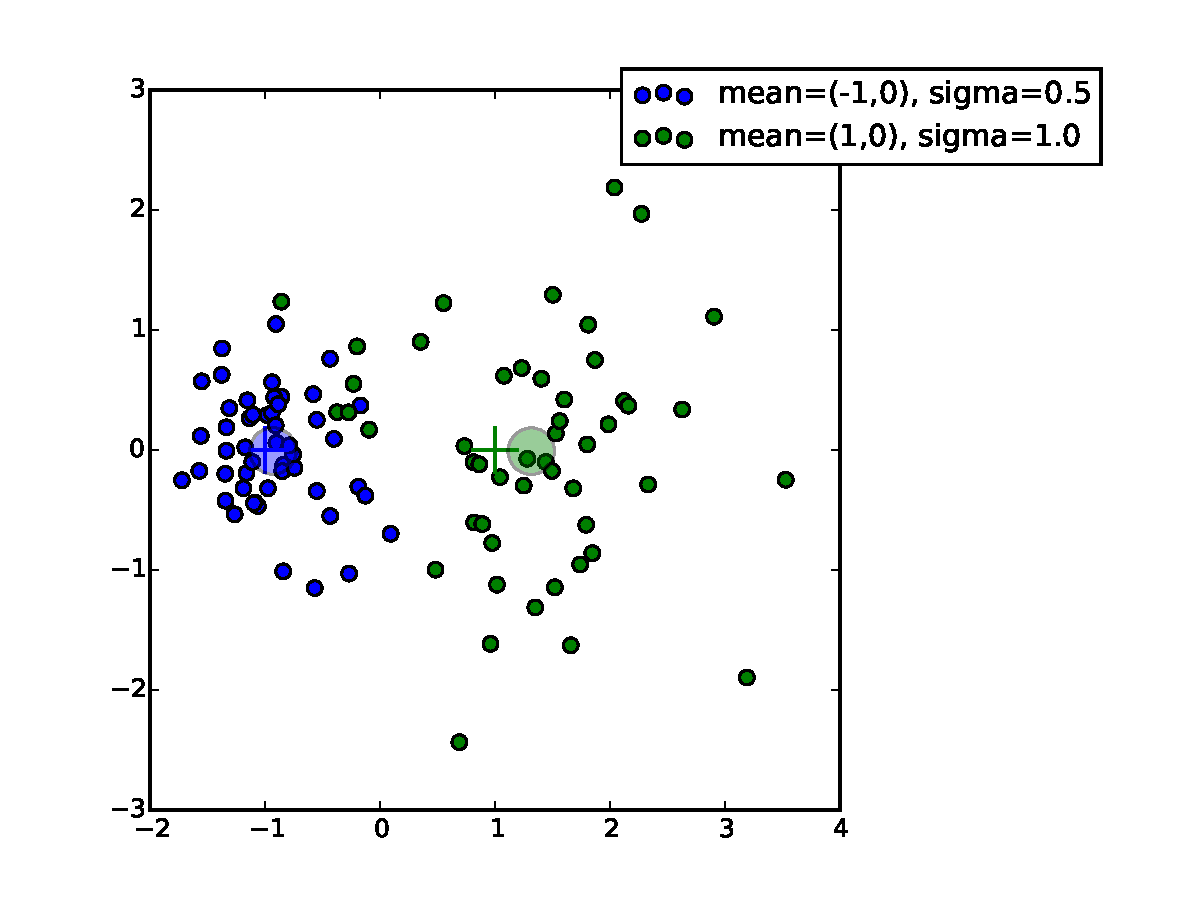
\includegraphics[page=1,width=\textwidth]{ex1.pdf}
\end{frame}
\begin{frame}{Example 1: naive attempt is not so bad\,\dots}
  \includegraphics[page=2,width=\textwidth]{ex1.pdf}
\end{frame}
\begin{frame}{Example 1: better with correction for pdf widths'}
  \includegraphics[page=3,width=\textwidth]{ex1.pdf}
\end{frame}


%%%%%%
\begin{frame}{Example 2: asymmetric gaussian distributions}
  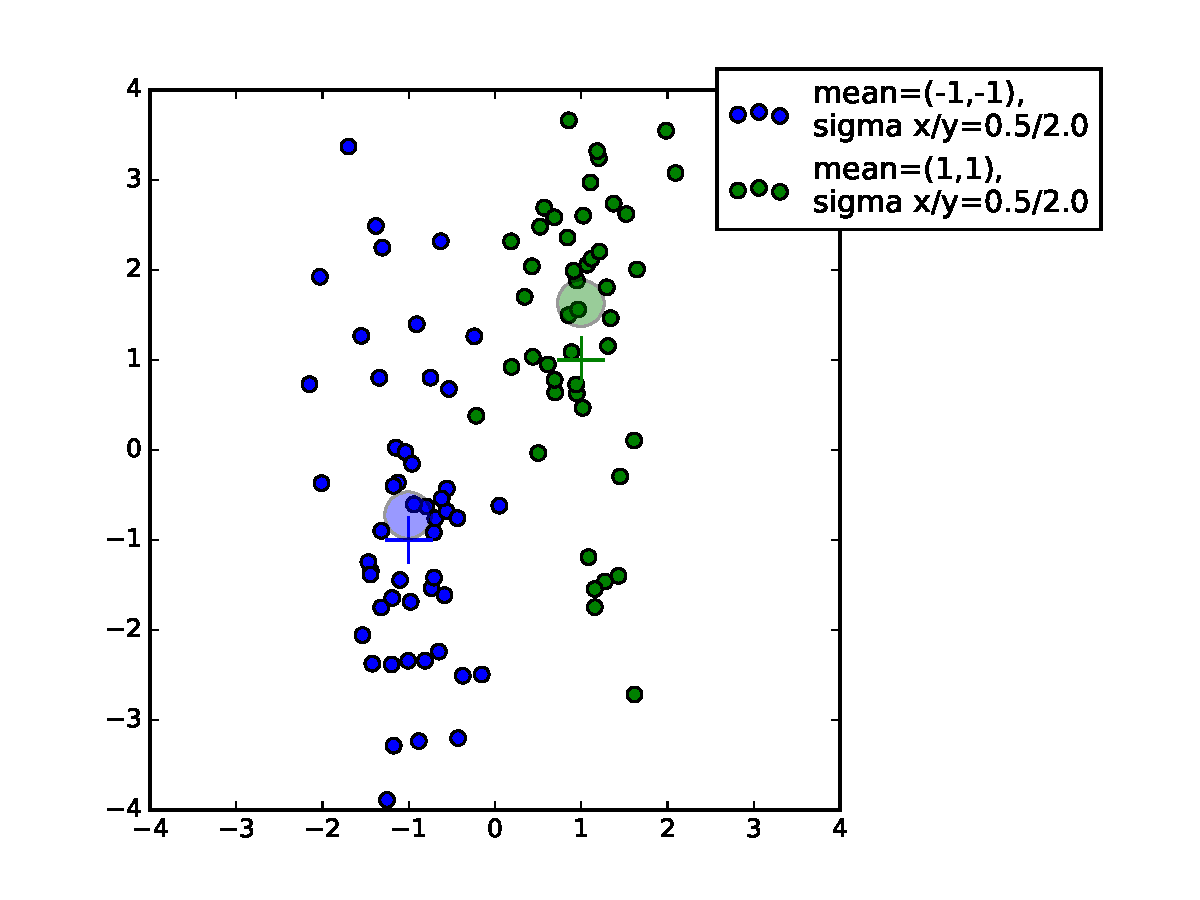
\includegraphics[page=1,width=\textwidth]{ex2.pdf}
\end{frame}
\begin{frame}{Example 2: naive attempt is worse\/\dots\,\dots}
  \includegraphics[page=2,width=\textwidth]{ex2.pdf}
\end{frame}
\begin{frame}{Example 2: classical Fisher classifier much better}
  \includegraphics[page=3,width=\textwidth]{ex2.pdf}
\end{frame}
\begin{frame}{Example 2: linear SVM classifier almost as good}
  \includegraphics[page=4,width=\textwidth]{ex2.pdf}
\end{frame}


%%%%%%
\begin{frame}{Fisher classifier}
  \begin{minipage}[c]{6cm}
    The idea was introduced by Ronald Fisher in his classic paper from 1936
    on discriminating three Iris flower species based on four anatomical measurements
    \href{https://en.wikipedia.org/wiki/Iris_flower_data_set}{\tt (Iris data)}

    \pause
    \begin{itemize}
    \item Consider the two class problem and seek the best dicriminating direction $\b w$
      in the observation space.
    \end{itemize}
  \end{minipage}
  \hfil
  \begin{minipage}[c]{4cm}
    \includegraphics[width=3.5cm]{Fisher.png}
    \par\noindent
    Ronald Fisher, 1890-1962
  \end{minipage}%
  \graphics{https://en.wikipedia.org/wiki/Ronald_Fisher}%
  \pause
  
  \begin{itemize}
  \item Let $\b m_1$ and $\b m_2$ denote estimated class means.
    It's natural to choose $\b w$ to maximize {\it inter-class separation} along $\b w$
    $$ \b w \cdot (\b m_2 - \b m_1) $$%

    \pause
  \item But then obviously $\b w \propto \b m_2 - \b m_1$ --- we just get the naive classifier!
    So another optimization criterium is added\dots
  \end{itemize}
\end{frame}


%%%%%%
\begin{frame}{Fisher classifier, continued}
  \begin{itemize}
  \item Let $\S_1$, $\S_2$ denote the corresponding estimated
    in-class covariance matrices.

    \pause
  \item Another natural objective while choosing $\b w$ is to minimize both of the
    {\it in-class variances\/} along $\b w$, or just the sum of these:
    $$ \b w \cdot \S_1 \b w + \b w \cdot \S_2 \b w
    = \b w \cdot (\S_1 + \S_2) \b w $$

    \pause
  \item The final optimization criterium is
    \begin{equation}  \label{eq:fisher}
      \argmax_{\b w}
      {(\b w\cdot \b m_{12})^2 \over \b w \cdot \S_{12} \b w}
    \end{equation}
    where $\b m_{12} =\b m_2 - \b m_1$ and $\S_{12} = \S_1 + \S_2$.

    \pause
  \item This can be interpreted as maximizing signal-to-noise ratio in the training data!

    \pause
  \item (Why do we absolutely need the square in the nominator?)
  \end{itemize}
\end{frame}
\def\eqfisher{\eqref{eq:fisher}}


%%%%%%
\begin{frame}{Fisher classifier, solution}
  \begin{itemize}
  \item The solution is found by equating the derivative to zero (some math involved):
    $$ \b w \propto \S_{12}^{-1}\b m_{12} $$
    %%\item TODO: Illustrate? Details on the classification boundary hyperplane?
    %%  Is Mahalanobis correction involved? Details of the derivation?

    \pause
  \item {\it Remark:\/} The idea behind \eqfisher\ may probably be applied
    in many new contexts. I like the appeal\/\dots
  \end{itemize}
  \vfill
  \vbox{}
\end{frame}


%%%%%%
\begin{frame}{Linear SVM}
  \begin{minipage}[c]{5.7cm}
    \begin{itemize}[<+->]
    \item A different approach to optimum separation\/\ldots
    \item The idea of {\it maximum-margin separating hyperplane\/} was developped
      by Vladimir Vapnik and others around 1964-65.
    \item The optimally separating hyperplane is based on {\it extreme\/}
      training observations which are called {\it support vectors\/} here.
    \end{itemize}
  \end{minipage}
  \hfil
  \begin{minipage}[c]{4.8cm}
    \includegraphics[width=4.8cm]{wiki-mmsh1.png}
  \end{minipage}
  \graphics{https://en.wikipedia.org/wiki/Support_vector_machine}%
  %https://en.wikipedia.org/wiki/Support_vector_machine#/media/File:Svm_separating_hyperplanes_(SVG).svg
  \pause

  \begin{itemize}
  \item {\it Side note:\/} classical perceptron learning algorithm may as well end up
    in $H_2$-like classifier. (Learning stops when all training examples are classified correctly.)
  %%\item {\it Remark:\/} This raises associations with a completely
  %%  different mathematical theory: Extreme Value Theory (EVT), the mathematical
  %%  theory of disasters.
  \end{itemize}
\end{frame}


%%% %%%%%%
%%% \begin{frame}{A diversion: remark on EVT}
%%%   \begin{minipage}[c]{6.0cm}
%%%     From S. Coles' book --- rainfall in south-east England
%%%     in years 1914-62.
%%% 
%%%     Estimation of probabilities of extreme values or the {\it tail\/}
%%%     of the distribution is obviously difficult.
%%%   \end{minipage}
%%%   \hfil
%%%   \begin{minipage}[c]{4.0cm}
%%%     \includegraphics[width=4.0cm]{opady01_Coles.png}
%%%   \end{minipage}
%%%   \pause
%%% 
%%%   \begin{itemize}
%%%   \item Standard parametric methods (MLE or the method of moments) are suited to estimation
%%%     of the distribution's body but are bad for the tail! Mainly due to data imbalance
%%%     (so little data in the tail) and required assumptions about the general shape
%%%     which may not hold for the tail.
%%% 
%%%     \pause
%%%   \item Empirical estimation of quantiles has this fundamental problem that the
%%%     probability of values greater then the maximum observed is\dots {\it zero!\/}
%%%     This is no good!
%%% 
%%%     \pause
%%%   \item EVT comes to the rescue: new limit theorems, universal limit distributions
%%%     --- beautiful math! But SVM also deals with extreme events!
%%%   \end{itemize}
%%% \end{frame}


%%%%%%
\begin{frame}{Linear SVM continued}
  \begin{minipage}[c]{5.9cm}
    \begin{itemize}
    \item Let $\b x_i\in\R^d,\ y_i\in\{-1, 1\}$, $i=1,2,\ldots N$
      denote the training data and targets.

      \pause
    \item We assume that the training data is linearly
      separable, so there exists a hyperplane
      $$ H: \b w \cdot \b x + b = 0, \ \|\b w\| > 0$$
      such that
      $$ y_i(\b w \cdot \b x_i + b) > 0,$$
      $i=1,2,\ldots N$
    \end{itemize}
  \end{minipage}
  \hfil
  \begin{minipage}[c]{4.7cm}
    \includegraphics[width=4.7cm]{wiki-mmsh2.png}
  \end{minipage}
  \graphics{https://en.wikipedia.org/wiki/Support_vector_machine}%
\end{frame}


%%%%%%
\begin{frame}{Linear SVM, optimization criterium}
  \begin{itemize}
  \item By appropriately scaling $\b w$ and $b$ we can assume that
    \begin{equation*} %%\label{eq:svm:constraint}
      y_i(\b w \cdot \b x_i + b) \ge 1, \ i=1,2,\ldots N
    \end{equation*}
    where the equality takes place
    for at least one observation from both the negative and positive class.

    \pause
  \item The margin for hyperplane $H$ is then equal to ${2/ \|\b w\|}$.
    (Recall that the distance from a point $\b x$ to $H$ is given by
    $ {|\b w \cdot \b x + b| / \|\b w\|} $.)

    \pause
  \item So the optimal $H$ is found by solving the following constrained
    minimization problem
    \begin{align}
      \label{eq:svm:pri:opt}
      {}& \argmin_{\b w,b}{1\over 2} \|\b w\|^2 \\
      \label{eq:svm:pri:constr}
      {}& y_i(\b w \cdot \b x_i + b) \ge 1, \ i=1,2,\ldots N
    \end{align}
  \end{itemize}
\end{frame}
\def\svmprimary{(\ref{eq:svm:pri:opt}-\ref{eq:svm:pri:constr})}


%%%%%%
\begin{frame}{Linear SVM, soft margin}
  \begin{itemize}[<+->]
  \item However, there are two issues with \svmprimary.
    \begin{itemize}
    \item the training set may not be linearly separable in the first place
    \item susceptability to outliers
    \end{itemize}
  \item So we allow to relax the constraint for individual training vectors and
    introduce a penalty for this
    \begin{align}
      \label{eq:soft:pri:opt}
      {}& \argmin_{\b \xi,w,b}\ {1\over 2} \|\b w\|^2 + C\sum_i \xi_i \\
      \label{eq:soft:pri:constr}
      {}& y_i(\b w \cdot \b x_i + b) \ge 1 - \xi_i, \ \xi_i\ge0, \ i=1,2,\ldots N
    \end{align}
  \item $C$ balances the cost of decreasing $\|\b w\|^2$ by introducing a positive $\xi_i$
    for some training vectors. (This is kind of $l_1$ regularization.)
  \end{itemize}
\end{frame}
\def\softprimary{(\ref{eq:svm:pri:opt}-\ref{eq:svm:pri:constr})}


%%%%%%
\begin{frame}{Linear SVM and convex optimization}
  \begin{itemize}
  \item For now we shall stick with non-regularized version, for simplicity.

    \pause
  \item Problem \svmprimary\ is a quadratic programming problem
    (minimization of a quadratic function subject to constraints involving
    inequalities with linear functions) for which solvers are available.

    \pause
  \item So problem solved\dots

    \pause
  \item Kind of\dots\ but a re-statement is beneficial!  %formulation

    \pause
  \item For an even more general class of {\it convex problems\/}:
    \begin{align}
      \label{eq:conv:pri:opt}
      {}& \argmin_{\b w}f(\b w) \\
      \label{eq:conv:pri:constr}
      {}& g_i(\b w) \le 0, \ i=1,2,\ldots N
    \end{align}
    where all functions $f$ and all $g_i$ are convex, the problem can be converted to 
    another --- a {\it dual problem}. 
  \end{itemize}
\end{frame}
\def\convprimary{(\ref{eq:conv:pri:opt}-\ref{eq:conv:pri:constr})}


%%%%%%
\begin{frame}{Lagrangian}
  \begin{itemize}
  \item We define the Lagrangian for problem \convprimary:
    \begin{equation*}
      \L(\b w,\alpha) = f(\b w) + \sum_i \alpha_i g_i(\b w), \ \
      \alpha_i\ge 0, \ i=1,2,\ldots N
    \end{equation*}
    
    \pause
  \item This is like Lagrangian for a problem with equality constraints
    (part of standard university calculus course), but here with additional
    constraints on the multipliers $\alpha_i$.
    
    \pause
  \item Consider the following quantity:
    \begin{equation*}
      \Theta(\b w) = \max_{\alpha:\,\forall_i\alpha_i\ge 0} \L(\b w, \alpha)
    \end{equation*}
    
    \pause
  \item The point is that (obvious!):
    \begin{equation*}
      \Theta(\b w) =
      \begin{cases}
        +\infty,\
        \hbox{\rm if $\b w$ violates any of the conditions \eqref{eq:conv:pri:constr}}\\
        f(\b w),\
        \hbox{otherwise}
      \end{cases}
    \end{equation*}
    
    \pause
  \item So we can replace problem \convprimary\ by the following:
    \begin{equation*}
      %\argmin_w \theta(w) = \argmin_w \max_{\alpha,\ \alpha_i\ge 0} \L(w, \alpha)
      \min_{\b w} \Theta(\b w) = \min_{\b w} \max_{\alpha:\,\forall_i\alpha_i\ge 0} \L(\b w, \alpha)
      \qquad ({}=\Theta_*)
    \end{equation*}
  \end{itemize}
\end{frame}


%%%%%%
\begin{frame}{Duality}
  \begin{itemize}
  \item How about changing the order of ``min'' and ``max''? The following inequality holds
    generally:
    \begin{equation*}
      (\theta^* = {})\quad
      \max_{\alpha:\,\forall_i\alpha_i\ge 0} \min_{\b w} \L(\b w, \alpha) \le
      \min_{\b w} \max_{\alpha:\,\forall_i\alpha_i\ge 0} \L(\b w, \alpha)
      \quad({}=\Theta_*)
    \end{equation*}

    \pause
  \item It's just because it holds {\it really\/} generally
    \begin{equation*}
      \max_x \min_y F(x,y) \le \min_y \max_x F(x, y)
    \end{equation*}
    for any function of two variables. Easy!

    \pause
  \item However the inverse inequality does not hold in this generality
    (consider $2xy/(x^2+y^2)$, $0<x,y<1$),
    so the inequality may in fact be strong for some function and variable domains.

    \pause
  \item Yet, for the problem \svmprimary, since minimized function is convex
    and constraints are affine, we have the equality $\theta^*=\Theta_*$.
  \end{itemize}
\end{frame}


%%%%%%
\begin{frame}{Duality continued}
  \begin{itemize}
  \item So the problem \svmprimary\ has an associated {\it dual problem}
    \begin{align}
      \label{eq:svm:dual:opt}
      {}& \argmax_\alpha \theta(\alpha) \\
      \label{eq:svm:dual:constr}
      {}& \alpha_i \ge 0, \ i=1,2,\ldots N
    \end{align}
    where
    \begin{equation*}
      \theta(\alpha) %% = \min_{\b w} \L(\b w, \alpha)
            = \min_{\b w, b} \left\{ {1\over 2} \|\b w\|^2
            + \sum_i \alpha_i\left[1 - y_i(\b w \cdot \b x_i + b) \right]
            \right\}
    \end{equation*}

    \pause
  \item The minimum with respect to $\b w$ can be computed by following standard
    ways. Equating the $(\b w,b)$-derivative to zero and solving for $\b w$ and $b$
    we get:
    \begin{align}
      \label{eq:svm:dual:w}
      {}& \b w = \sum_i\alpha_iy_i\b x_i \\
      \label{eq:svm:dual:b}
      {}& \sum_i\alpha_iy_i=0
    \end{align}
  \end{itemize}
\end{frame}


%%%%%%
\begin{frame}{Dual problem final form}
  \begin{itemize}[<+->]
  \item Substituting back we get the following expression for $\theta$:
    \begin{equation}
      \label{eq:svm:dual:theta2}
      \theta(\alpha) = 
      \sum_i\alpha_i
      - {1\over 2}\sum_{ij}y_iy_j\alpha_i\alpha_j\,\b x_i\cdot\b x_j,
      \quad \sum_i\alpha_iy_i=0
    \end{equation}
  \item and the formulation of the dual problem:
    \begin{equation}
      \label{eq:svm:dual:opt2}
      \argmax_\alpha \theta(\alpha), \quad
      \sum_i\alpha_iy_i=0, \quad \alpha_i \ge 0, \ i=1,2,\ldots N
    \end{equation}
  \item and the decision criterium for unseen $\b x$:  %%\eqref{eq:svm:dual:w}
    \begin{align}
      \label{eq:svm:dual:rule2}
      & f(\b x) = \b w \cdot \b x + b = \sum_i\alpha_iy_i\,\b x_i\cdot \b x + b\\
      \nonumber
      & b = - (1/2)\big(\max_{i:y_i=-1}\b w\cdot\b x_i + \min_{i:y_i=1}\b w\cdot\b x_i\big)
    \end{align}
  \item Since the solution of \eqref{eq:svm:dual:opt2} yields all $\alpha_i$ zero except
    for a small number of support vectors, the sum and min/max in \eqref{eq:svm:dual:rule2}
    are restricted to only a small number of indexes, say $i\in S$.
  \end{itemize}
\end{frame}


%%%%%%
\begin{frame}{Why bother about duality?}
  \begin{itemize}[<+->]
  \item But finally, what's the real gain in moving from primary to dual problem in SVM?
  \item There is a specialized and very effective algorithm for solving this particular
    QP problem: the sequential minimal optimization (SMO) algorithm. (Not part of this
    presentation.)
  \item But I also like an answer I saw somewhere in the Web.
    \begin{itemize}[<+->]
    \item short one: {\it kernels!}
    \item longer: {\it keeerneeeels!}
    \end{itemize}
  \item The nice property of the dual problem and decision criterium is that the
    training data appears exclusively in the form of scalar products $\b x_i\cdot \b x_j$.
  \item This allows for easy replacement of raw observations by {\it features}\dots\
    Possibly very high-dimensional ones.
  \item And features are connected to kernels\dots
  \end{itemize}
\end{frame}


%%%%%%
\begin{frame}{Nonlinear classification problems}
  \begin{minipage}[c]{6.2cm}
    \begin{itemize}[<+->]
    \item Some classification problems can't be
      solved with linear methods --- notably the XOR problem.
    \item Regardless that the training data is not linearly
      separable in the original {\it observation space\/}
      this is ``easily'' overcome by introducing an extra
      {\it feature\/} $\phi(\b x)=x_1x_2$.
    \end{itemize}
  \end{minipage}
  \hfil
  \begin{minipage}[c]{4.4cm}
    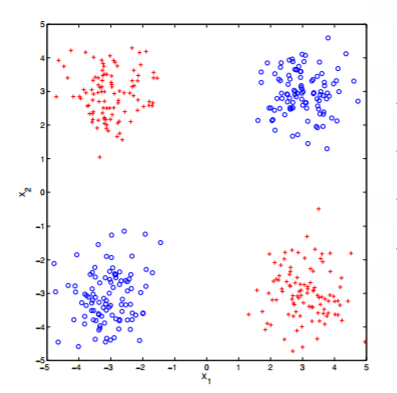
\includegraphics[width=4.3cm]{xor.png}
  \end{minipage}
  \begin{itemize}[<+->]
  \item When mapped to a higher dimensional feature space with
    $$ (x_1,x_2) \mapsto (X_1,X_2,X_3)=\Phi(x_1,x_2)=(x_1,x_2,x_1x_2) $$
    the data is separable with $X_3=0$ hyperplane (or some other which may be even
    more optimal for the data).
  \item The resulting classification boundary in the observation space is nonlinear.
  \end{itemize}
\end{frame}


%%%%%%
\begin{frame}{SVM with features}
  \begin{itemize}[<+->]
  \item Assume that we have feature set $\R^d\ni\b x\mapsto \Phi(\b x)\in\R^D$.
    %%\begin{equation*}
    %%  \R^d\ni\b x\mapsto \Phi(\b x)\in\R^D
    %%\end{equation*}
  \item There may be a lot of features ($D$ much bigger than $d$), but they are great in separating training data!
  \item To run SVM with features rather than original observations, it suffices
    to replace $\b x$'s by $\Phi(\b x)$'s in
    \eqref{eq:svm:dual:theta2}, \eqref{eq:svm:dual:opt2} and \eqref{eq:svm:dual:rule2}.
  \item Note that we now need no structure in the observation space --- no
    geometry, distance, scalar products, hyperplanes,\dots\ So it can be just a plain set $\X$ instead of $\R^d$.
    Only the feature space counts now and the performance of features.
  \item Two {\it little\/} problems\dots
  \item A lot of features result in more workload, like $O(D^2)$.
  \item How to develop good feature set?
  \item Interestingly both of them can be addressed with {\it kernels}\dots
  \end{itemize}
\end{frame}


%%%%%%
\begin{frame}{From features to kernel \dots}
  \begin{itemize}[<+->]
  \item With a feature map $\Phi:\X\to\R^D$ we can define a 2-variable function:
    \begin{equation}
      \label{eq:kernel:fromfeatures}
      K:\X\times\X\to\R,\quad K(\b x, \b x')=\Phi(\b x)\cdot\Phi(\b x')
    \end{equation}
  \item Obviously $K$ is symmetric: 
    \begin{equation}
      \label{eq:kernel:symmetry}
      \forall_{\b x, \b x' \in\X} K(\b x, \b x') = K(\b x', \b x)
    \end{equation}
  \item And the following property is quite easy to verify:
    \begin{equation}
      \label{eq:kernel:positive}
      \forall_n \forall_{\b x_1,\b x_2,\ldots\ \b x_n\in\X}
      \forall_{\alpha_1,\alpha_2,\ldots\ \alpha_n\in\R}
      \sum_{i,j=1}^n \alpha_i\alpha_jK(\b x_i,\b x_j) \ge 0
    \end{equation}
  \item (\/The sum is equal to $\b X\cdot\b X$, where $\b X=\sum_i\alpha_i\Phi(\b x_i)$.\/)
  \item We call $K$ a (symmetric, positive-definite) {\it kernel\/} on $\X$.
  \end{itemize}
\end{frame}
\def\iskernel{(\ref{eq:kernel:symmetry}-\ref{eq:kernel:positive})}


%%%%%%
\begin{frame}{\dots\ and back}
  \begin{itemize}[<+->]
  \item Assume $K$ is a kernel on $\X$, so that \iskernel\ hold. Then, with some additional more theoretical
    assumptions, there exists a mapping $\Phi:\X\to H$, where $H$ is a space with a scalar product, such that
    \begin{equation*}
      K(\b x, \b x')=\Phi(\b x)\cdot\Phi(\b x')
    \end{equation*}
  \item The little catch here is that the space $H$ may be infinite dimentional
    and $\cdot$ is the scalar product in $H$ --- a kernel is generally associated with infinitely many features.
  \item So $H$ is a {\it Hilbert\/} space\dots\ But do we care?
  \item No! Because we don't have to see features and compute the scalar products explicitely --- 
    the kernel computes them for us!
  \item About the ``additional assumptions''\dots\ These may be: let $\X$ be a compact
    topological space with a strictly positive finite Borel measure and $K$ be continues.
    Or just $X=[a,b]$ and $K$ continues. For the curious: see {\it Mercer's theorem}.
  \end{itemize}
\end{frame}


%%%%%%
\begin{frame}{Kernel SVM}
  \begin{align*}
    & \theta(\alpha) = 
    \sum_i\alpha_i
    - {1\over 2}\sum_{ij}y_iy_j\alpha_i\alpha_j\,K(\b x_i,\b x_j),
    \quad \sum_i\alpha_iy_i=0 \\[10pt]
    & \argmax_\alpha \theta(\alpha), \quad
    \sum_i\alpha_iy_i=0, \quad \alpha_i \ge 0, \ i=1,2,\ldots N \\[10pt]
    & f(\b x) = \sum_{i\in S}\alpha_i y_i\,K(\b x_i,\b x) + b\\
    & \qquad b = - (1/2)\big(\max_{i\in S:y_i=-1}f_0(\b x_i) + \min_{i\in S:y_i=1}f_0(\b x_i)\big),\\
    & \qquad f_0(x_i) = \sum_{j\in S}\alpha_j y_j\,K(\b x_j,\b x_i)
  \end{align*}
  \begin{itemize}[<+->]
  \item Note that $K(\b x_i,\b x_j)=K_{ij}$ is just a matrix
    (symmetrical and positive-semidefinite).
  \end{itemize}
\end{frame}


%%%%%%
\begin{frame}{Kernel SVM, continued}
  \begin{itemize}[<+->]
  \item Kernel SVM was developped by Vapnik and co-workers in 1992-95:
    \begin{itemize}
    \item Initial paper introducing the algorithm:
      \href{http://www.svms.org/training/BOGV92.pdf}{Boser, Guyon and Vapnik, 1992}
    \item Matched performance on MNIST with CNN at the time:
      \href{http://image.diku.dk/imagecanon/material/cortes_vapnik95.pdf}{Cortes and Vapnik, 1995}
    \end{itemize}
  \item Results on MNIST in 1995:
    \begin{itemize}[<+->]
    \item Test error for SVM: 1.1\%. LeNet-1: 1.7, LeNet-4: 1.1.
    \item However LeNet-4 was carefully handcrafted based on the errors made by a long standing
      state-of-the-art LeNet-1 (since 1989)
    \item SVM was not engineered in a similar fashion, citation from
      \href{http://yann.lecun.com/exdb/publis/pdf/lecun-98.pdf}{LeCun et. al., 1998}:\\
      {\it
      The SVM has excellent accuracy, which is most remarkable, because unlike the other
      high preformance classifiers it does not include a priori knowlegde about the problem.
      In fact, this classifier would do just as well if the image pixels were permuted
      with a fixed mapping and lost their pictorial structure.}
    %%% \item (LeNet-1 and LeNet-4 were superceeded by a larger network LeNet-5 in 1998.
    %%%   Main reason why larger models were not considered earlier was the amount of training data
    %%%   available.)
    \end{itemize}
  \end{itemize}
\end{frame}


%%%%%%
\begin{frame}{Kernel SVM, continued}
  \begin{itemize}[<+->]
  \item Interestingly SVM (and kernel methods in general) became the mainstream machine learning
    algorithm in late 1990's early 2000's and the interest in ANN's decreased considerably.
  \item Things changed again around 2010.
  \item Maybe it's good to remember this?
  \item A little curiosity from speech domain, not so old:
    \href{https://pdfs.semanticscholar.org/3cc7/230bd445128fc0dfb62cf54bfb01c25d377c.pdf}%
         {Huang, Avron, Sainath, Sindhwani, Ramabhadran,
           {\it Kernel methods match deep neural networks on TIMIT}, 2014.}\\
         (Most of the authors from IBM T.J. Watson Research Center. It's not about SVM but
         {\it randomized approximate feature maps\/} generated with kernels\/\ldots\ But not today!)

  \end{itemize}
\end{frame}


%%%%%%
\begin{frame}{What kernel?}
  \begin{itemize}[<+->]
  \item The intuition is that the kernel is a {\it similarity measure\/} in the observation
    space. This similarity measure implies features.
  \item Anyway, the choice of the kernel is the tricky part! Apart from regularization weight\/\ldots\
    Some example kernels:
    \begin{itemize}[<+->]
    \item Polynomial kernel with degree $p$:
      $$ K(\b x,\b x') = (\b x\cdot\b x' + c)^p, \quad c>=0,\ p\in\N $$
    \item Radial basis function (or gaussian) kernel:
      $$ K(\b x, \b x') = \exp(-\|\b x-\b x'\|^2/2\sigma^2), \quad \sigma>0 $$
    \item And of course many more, also of a different taste: string kernels for text
      classification, graph kernels, Fisher information kernels,
      locality improved kernels,\/\dots\ One can also construct kernels from other kernels.
    \end{itemize}
  \item Some try to learn the kernel from the data\/\ldots
  \end{itemize}
\end{frame}


%%%%%%
\begin{frame}{Example 3: Iris data, PCA transformed}
  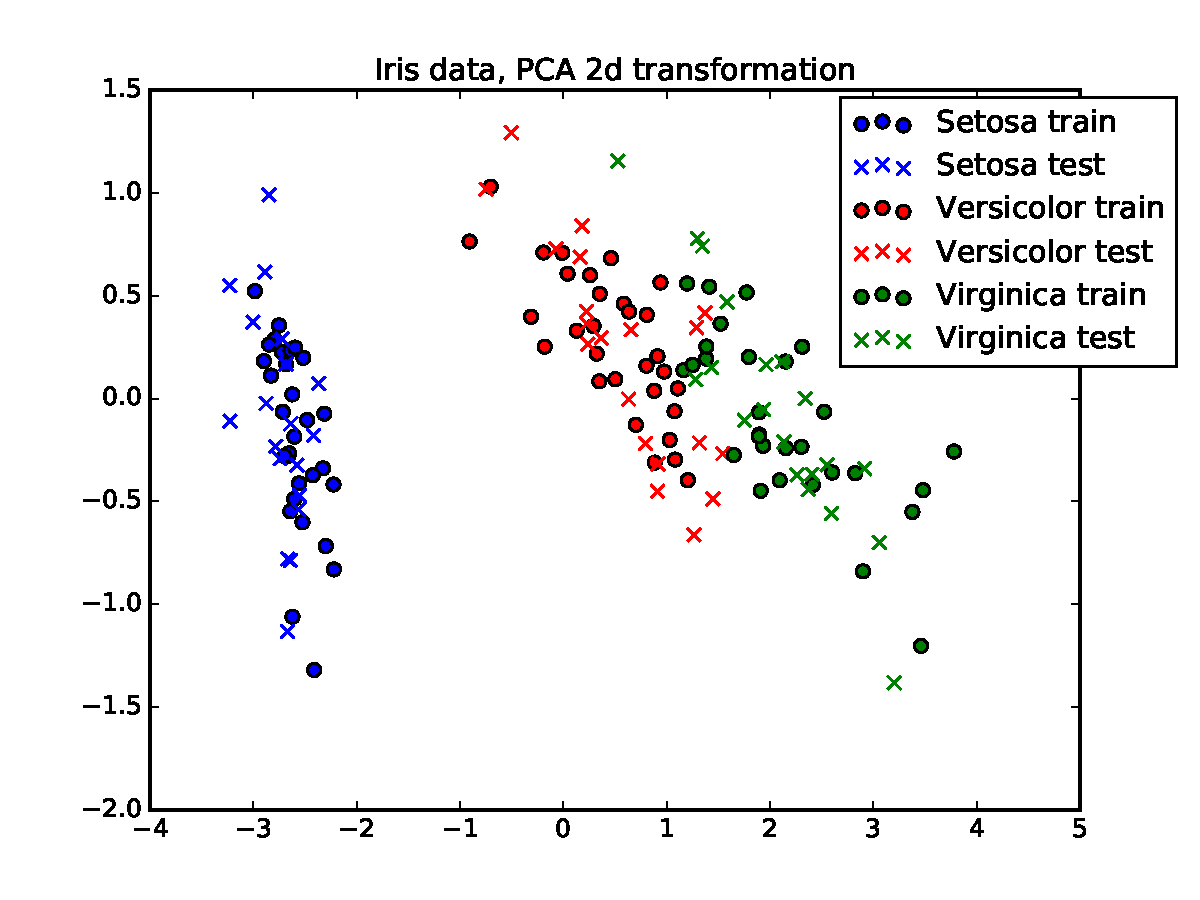
\includegraphics[page=1,width=\textwidth]{iris_svm.pdf}
\end{frame}
\begin{frame}{Example 3: Versicolor vs Virginica, Fisher classifier}
  \includegraphics[page=2,width=\textwidth]{iris_svm.pdf}
\end{frame}
\begin{frame}{Example 3: Versicolor vs Virginica, linear SVM}
  \includegraphics[page=3,width=\textwidth]{iris_svm.pdf}
\end{frame}
\begin{frame}{Example 3: Versicolor vs Virginica, cubic SVM}
  \includegraphics[page=4,width=\textwidth]{iris_svm.pdf}
\end{frame}
\begin{frame}{Example 3: Versicolor vs Virginica, gaussian SVM}
  \includegraphics[page=5,width=\textwidth]{iris_svm.pdf}
\end{frame}
\begin{frame}{Example 3: Versicolor vs Setosa+Virginica, square SVM}
  \includegraphics[page=6,width=\textwidth]{iris_svm.pdf}
\end{frame}


%%%%%%
\begin{frame}{Kernel methods: high level view}
  \begin{itemize}[<+->]
  \item The basic idea is:
    \begin{itemize}[<+->]
    \item Choose a kernel $K(\b x, \b x')$ and thus the implicit feature map
      $\Phi(\b x)$. No need to see/derive any explicit formula for $\Phi$!
    \item Solve the underlying {\it linear\/} problem in the feature space. As long as
      the solution involves only scalar products of features of training data,
      the kernel $K$ will suffice.
    \item Map the solution back to original observation space --- done!
    \end{itemize}
  \item Many examples: kernel SVM, kernel PCA, kernel DA (kernelized LDA), \dots
  \item Consider PCA. The linear classics works like this:
    assume that we have zero centered training data
    $(1/N)\sum_n {\b x}_n=0$ we compute the covariance matrix
    $\C=(1/N)\sum_n{\b x}_n{\b x}_n^T=$,
    which is symmetric. Then we solve the eigenvalue problem $\C{\b x}=\lambda{\b x}$.
    Eigenvectors of largest eigenvalues indicate principal directions.
  \item Let's take a look at the kernelized version\/\ldots\ (Some details are skipped.
    For example: how to ensure zero centering in the feature space? See
    \href{ftp://ftp.cfar.umd.edu/.snapshot/hourly.2/pub/aravinds/scholkopf98-kernel.pdf}%
         {Sch\"olkopf et.al 1998})
  \end{itemize}
\end{frame}


%%%%%%
\begin{frame}{Kernel PCA, the algorithm}
  \begin{itemize}[<+->]
    \item For the kernel version the underlying feature space problem is
      $$ \C{\b V}=\lambda{\b V}, \ \C={1\over N}\sum_n{\b V}_n{\b V}_n^T, \ {\b V}_n=\Phi({\b x}_n) $$
    \item Since $\C{\b V}=(1/N)\sum_n({\b V}_n\cdot{\b V}){\b V}_n$ the eigenvectors are spanned by ${\b V}_n$
      so it's sufficient to compute the coefficients ${\b V}=\sum_na_n{\b V}_n$. We rewrite the eigenvalue problem
      like so:
      $$ {\b V}_m\cdot\C{\b V} = {1\over N}\sum_n({\b V}_n\cdot{\b V}_m)({\b V}_n\cdot{\b V})
      = {1\over N}\sum_n \K_{nm}a_n $$
      where $\K_{mn}={\b V}_m\cdot(\b V)_n=K({\b x}_m, {\b x}_n)$ and since the right hand side is then
      $\lambda a_m$ we get $(1/N)\sum_n \K_{nm}a_n=\lambda a_m$. Finally ($\K$ is symmetric):
      $$ \K{\b a}=N\lambda {\b a} $$
    \item Projection onto eigenvector (corresponding to) ${\b a}$ is given by
      $$ (\sum_n a_n{\b V}_n)\cdot{\b V} = \sum_n a_nK({\b x}_n,{\b x}) $$
  \end{itemize}
\end{frame}


%%%%%%
\begin{frame}{Example 4: Iris data, kernel PCA}
  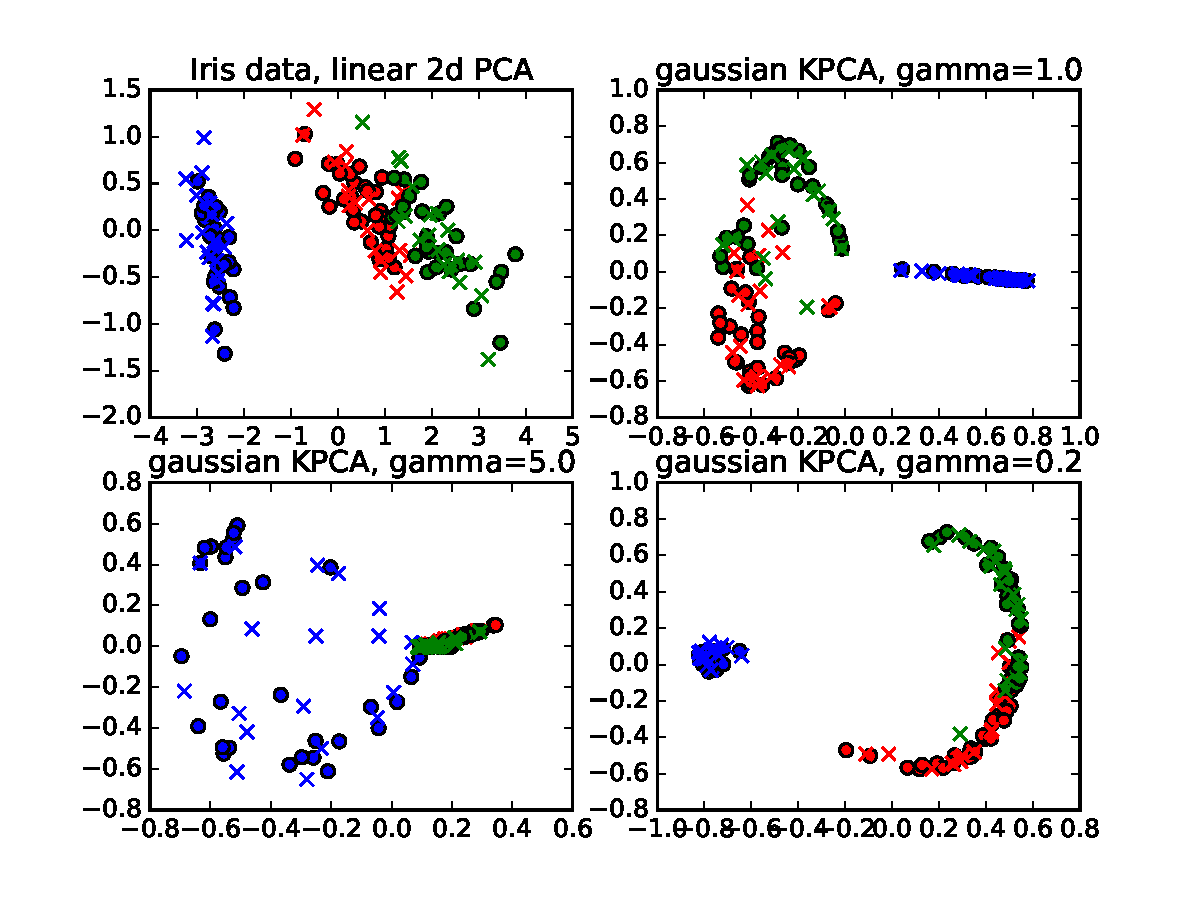
\includegraphics[page=1,width=\textwidth]{iris_kernel.pdf}
\end{frame}


%%%%%%
\begin{frame}{Example 5: KPCA example from Wikipedia}
  \includegraphics[width=\textwidth]{Kernel_pca_input.png}
\end{frame}
\begin{frame}{Example 5: KPCA with square polynomial kernel}
  \includegraphics[width=\textwidth]{Kernel_pca_output.png}
\end{frame}
\begin{frame}{Example 5: KPCA with gaussian kernel}
  \includegraphics[width=\textwidth]{Kernel_pca_output_gaussian.png}
\end{frame}


%%%%%%
\begin{frame}{Wikipedia credits}

  {\small
    
    \url{https://commons.wikimedia.org/w/index.php?curid=42169073}\\
    by Flikr commons
    \url{https://www.flickr.com/photos/internetarchivebookimages/20150531109/}, CC BY 2.0

    \medskip

    \url{https://commons.wikimedia.org/w/index.php?curid=22877598}\\ 
    by User:ZackWeinberg, based on PNG version by User:Cyc, CC BY-SA 3.0

    \medskip

    \url{https://commons.wikimedia.org/w/index.php?curid=3566688}\\
    by Cyc --- Own work, Public Domain

    \medskip

    \url{https://commons.wikimedia.org/w/index.php?curid=3936385}\\
    by Petter Strandmark --- Own work, CC BY 3.0

    \smallskip

    \url{https://commons.wikimedia.org/w/index.php?curid=3936390}\\
    by Petter Strandmark --- Own work, CC BY 3.0 

    \smallskip

    \url{https://commons.wikimedia.org/w/index.php?curid=3936753}\\
    by Petter Strandmark --- Own work, CC BY 3.0 

  }
  
\end{frame}


%%% %%%%%%
%%% \begin{frame}{Examples}
%%%   \includegraphics[width=\textwidth]{iris.png}
%%% \end{frame}
%%% \begin{frame}{Examples}
%%%   \includegraphics[width=\textwidth]{iris-lin.png}
%%% \end{frame}
%%% \begin{frame}{Examples}
%%%   \includegraphics[width=\textwidth]{iris-poly2.png}
%%% \end{frame}
%%% \begin{frame}{Examples}
%%%   \includegraphics[width=\textwidth]{iris-poly10.png}
%%% \end{frame}
%%% \begin{frame}{Examples}
%%%   \includegraphics[width=\textwidth]{iris-radial.png}
%%% \end{frame}
      


\end{document}
%%%%%%%%%%%%%%%%%%%%%%%%%%%%%%%%%%

%%%%%%
\begin{frame}{TODO}
  \begin{itemize}[<+->]
  \item TODO
  \end{itemize}
\end{frame}

\begin{equation}
\end{equation}

\begin{align}
\end{align}
